% Document setup
\documentclass[12pt]{article}
\usepackage[margin=1in]{geometry}
\usepackage{fancyhdr}
\usepackage{lastpage}

\pagestyle{fancy}
\lhead{Richard Whitehill}
\chead{PHYS 804 -- HW \HWnum}
\rhead{\duedate}
\cfoot{\thepage \hspace{1pt} of \pageref{LastPage}}

% Encoding
\usepackage[utf8]{inputenc}
\usepackage[T1]{fontenc}

% Math/Physics Packages
\usepackage{amsmath}
\usepackage{amssymb}
\usepackage{mathtools}
\usepackage{physics}
\usepackage{siunitx}

\AtBeginDocument{\RenewCommandCopy\qty\SI}

% Enumeration/itemize
\usepackage{enumitem}
\newenvironment{parts}
{\begin{enumerate}[label=\textbf{(\alph*)},leftmargin=*,itemsep=-10pt]
}{\end{enumerate}}

% Reference Style
\usepackage{hyperref}
\hypersetup{
    colorlinks=true,
    linkcolor=blue,
    filecolor=magenta,
    urlcolor=cyan,
    citecolor=green
}

\newcommand{\eref}[1]{Eq.~(\ref{eq:#1})}
\newcommand{\erefs}[2]{Eqs.~(\ref{eq:#1})--(\ref{eq:#2})}

\newcommand{\fref}[1]{Fig.~\ref{fig:#1}}
\newcommand{\frefs}[2]{Figs.~\ref{fig:#1}--\ref{fig:#2}}

\newcommand{\tref}[1]{Table~\ref{tab:#1}}
\newcommand{\trefs}[2]{Tables~\ref{tab:#1}-\ref{tab:#2}}

% Figures and Tables 
\usepackage{graphicx}
\usepackage{float}
\usepackage[font=small,labelfont=bf]{caption}

\newcommand{\bef}{\begin{figure}[h!]\begin{center}}
\newcommand{\eef}{\end{center}\end{figure}}

\newcommand{\bet}{\begin{table}[h!]\begin{center}}
\newcommand{\eet}{\end{center}\end{table}}

% tikz
\usepackage{tikz}
\usetikzlibrary{calc}
\usetikzlibrary{decorations.pathmorphing}
\usetikzlibrary{decorations.markings}
\usetikzlibrary{arrows.meta}
\usetikzlibrary{positioning}
\usetikzlibrary{3d}
\usetikzlibrary{shapes.geometric}

% tcolorbox
\usepackage[most]{tcolorbox}
\usepackage{xcolor}
\usepackage{xifthen}
\usepackage{parskip}

\newcommand*{\eqbox}{\tcboxmath[
    enhanced,
    colback=black!10!white,
    colframe=black,
    sharp corners,
    size=fbox,
    boxsep=8pt,
    boxrule=1pt
]}

% problem-solution macros
% \usepackage{adjustbox}
\usepackage{changepage}

\newtcolorbox{probbox}[1][]{
    breakable,
    enhanced,
    boxrule=0pt,
    frame hidden,
    borderline west={4pt}{0pt}{green!50!black},
    colback=green!5,
    before upper=\textbf{Problem #1) \,},
    % \textbf{Problem #1 \ifthenelse{\isempty{#1}}{}{: #1} \\ },
    sharp corners,
    parbox=false
}

% \newtcolorbox{ProblemBox}[1][]{%
%   breakable,
%   enhanced,
%   colback=black!10!white,
%   colframe=black,
%   title={\large #1 \hfill}
% }
\newcommand{\prob}[2]{
\begin{probbox}[#1]
#2
\end{probbox}
}

\newenvironment{solution}{\begin{adjustwidth}{8pt}{8pt}}{\end{adjustwidth}}
\newcommand{\sol}[1]{
\begin{solution}
#1
\end{solution}
}
% \textbf{#1)} #2}

% Miscellaneous Definitions/Settings
\newcommand{\reals}{\mathbb{R}}
\newcommand{\integers}{\mathbb{Z}}
\newcommand{\naturals}{\mathbb{N}}
\newcommand{\rationals}{\mathbb{Q}}
\newcommand{\complexs}{\mathbb{C}}

\setlength{\parskip}{\baselineskip}
\setlength{\parindent}{0pt}
\setlength{\headheight}{14.49998pt}
\addtolength{\topmargin}{-2.49998pt}


\def\HWnum{Final}
\def\duedate{December 13, 2024}

\usepackage{slashed}

\begin{document}

\prob{1}{

Consider the classical Lagrangian densities for the following relativistic quantum field theories,
\begin{align}
\label{eq:LY}
\mathcal{L}_{Y} &= \frac{i}{2} \bar{\psi} \overleftrightarrow{\slashed{\partial}} \psi - M \bar{\psi} \psi + \frac{1}{2} (\partial \phi)^2 - \frac{1}{2} m_{s}^2 \phi^2 - g \bar{\psi} \psi \phi - \frac{\lambda_{1}}{3!} \phi^3 - \frac{\lambda_2}{4!} \phi^{4} \\
\label{eq:LV}
\mathcal{L}_{V} &= \frac{i}{2} \bar{\psi} \overleftrightarrow{\slashed{\partial}} \psi - M \bar{\psi} \psi - \frac{1}{4} F^{\mu\nu} F_{\mu\nu} + \frac{m_{V}^2}{2} A^{\mu} A_{\mu} - g \bar{\psi} \slashed{A} \psi
.\end{align}
We could envision each of these being proposed as moels of the interactions between spinor ``nucleons'' of mass $M$ represented by the Fermi field $\psi$.
In the first case, the interaction is then mediated by a scalar ``pion'' field $\phi$ with mass $m_{s}$, and in the second it is mediated by a vector field $A^{\mu}$ with mass $m_{V}$.
As usual, the field strength tensor $F^{\mu\nu} = \partial^{\mu} A^{\nu} - \partial^{\nu} A^{\mu}$.
(Note that to be realistic we should really have \underline{pseudo}scalar and vector interactions.)
In the second theory, we would get the Maxwell field if we set $m_{V} = 0$.

\begin{parts}

\item Use the fast mnemonic that we developed in class for translating a classical Lagrangian density into QFT Feynman rules to write down all the Feynman rules for the two theories above.
    Make a comment about where each factor of ``$i$'' comes from.
    Use straight lines for $\psi$, dashed lines for $\phi$, and wavy lines for $A^{\mu}$.

\item Draw a two-loop diagram for the vector field case.
    Draw an example of a diagram that would give problems if you have not worried about the ``reduction'' of external leg states.

\item What happens if we then place $m_{V} = 0$ in the vector field?
    A standard way to deal with the problem is to replace $\frac{m_{V}^2}{2} A_{\mu} A^{\mu} \rightarrow -\frac{1}{2 \xi} (\partial_{\mu} A^{\mu})^2$.
    This effectively uses the Lagrange multiplier technique to fix the Lorenz gauge condition $\partial_{\mu} A^{\mu} = 0$.
    What are the Feynman rules if I make this replacement?
    What if I further specify the gauge by fixing $\xi = 1$, where $\xi$ is a real constant that will be chosen later?

\item Using Eq. (\ref{eq:LY}), draw all the Feynman diagrams that would contribute to the $2 \rightarrow 2$ cross section, $\psi \bar{\psi} \rightarrow \psi \bar{\psi}$ \underline{through} order $g^2$ and $g^2 \lambda_1^2$.

\item Still using Eq. (\ref{eq:LY}), consider the cross section for the $2 \rightarrow 2$ scattering process $\psi \psi \rightarrow \psi \psi$.
    Start with the general cross section expression derived in class,
    \begin{align}
        \dd{\sigma} = \frac{|M|^2}{2 \sqrt{\lambda(s,m_{A}^2,m_{B}^2)}} \frac{\dd[3]{\vb*{p}_{1}}}{(2 \pi)^3 2 E_{1}} \ldots \frac{\dd[3]{\vb*{p}_{N}}}{(2 \pi)^3 2 E_{N}} (2 \pi)^{4} \delta\Big( k_{A} + k_{B} - \sum_{i=1}^{N} p_{i} \Big)
    ,\end{align}
    with
    \begin{align}
        \lambda(s,m_{A}^2,m_{B}^2) = s^2 + m_{A}^{4} + m_{B}^{4} - 2 s m_{A}^2 - 2 s m_{B}^2 - 2 m_{A}^2 m_{B}^2
    ,\end{align}
    and derive the order $g^2$ expression for the unpolarized differential cross section $\dv*{\sigma}{\Omega}|_{\rm CM}$ in the center-of-mass system.
    Since it is an unpolarized cross section, you should sum over the final and average over initial nucleon spins.
    Let $p_{A}$ and $p_{B}$ label the initial four-momenta and $p_{C}$ and $p_{D}$ label the final four-momenta and express your result in terms of Mandelstam variables.
    
\end{parts}

}

\sol{

(a) Let us rewrite the Yukawa and vector Lagrangians as follows:
\begin{align}
    \mathcal{L}_{Y} &= \mathcal{L}_{D,\rm sym} + \mathcal{L}_{\rm KG} - g \bar{\psi} \psi \phi - \frac{\lambda_1}{3!} \phi^3 - \frac{\lambda_2}{4!} \phi^{4} \\
    \mathcal{L}_{V} &= \mathcal{L}_{D,\rm sym} + \mathcal{L}_{\rm P} - g \bar{\psi} \slashed{A} \psi
,\end{align}
where $\mathcal{L}_{D,\rm sym} = \bar{\psi} (\frac{i}{2} \overleftrightarrow{\slashed{\partial}} - M ) \psi$ is the free Dirac Lagrangian for spin-1/2 spinor fields, $\mathcal{L}_{KG} = \frac{1}{2} \partial_{\mu} \phi \partial^{\mu} \phi - \frac{m_{s}^2}{2} \phi$ is the free Klein-Gordon Lagrangian for real scalar particles, and $\mathcal{L}_{P} = -\frac{1}{4} F^{\mu\nu} F_{\mu\nu} + \frac{m_{V}^2}{2} A^{\mu} A_{\mu}$ is the free Proca Lagrangian for a spin-1 vector particles.
The vertices are simple enough to read from the Lagrangian since they are just the coefficients without any factor included for symmetries multiplied by $i$.
We can determine the propagators easily enough from the mnemonic.
For the KG scalar propagator, we list out the steps as follows:
\begin{gather}
    D = [ (i p_{\mu}) (-i p^{\mu}) - m_{s}^2 ] = p^2 - m_{s}^2 \rightarrow D^{-1} = \frac{1}{p^2 - m_{s}^2 + i \epsilon} \rightarrow {\rm Prop} = \frac{i}{p^2 - m_{s}^2 + i \epsilon}
.\end{gather}
Similarly, we can determine the Dirac propagator
\begin{align}
    D = \frac{i}{2} \gamma^{\mu} [ (-i p_{\mu}) - (i p_{\mu}) ] - M = \slashed{p} - M \rightarrow {\rm Prop} = \frac{i}{\slashed{p} - M} = \frac{i (\slashed{p} + M)}{p^2 - M^2 + i \epsilon}
.\end{align}
For the Proca theory, we must massage the Lagrangian a bit to arrive at a form where we can use the mneumonic properly:
\begin{align}
    \mathcal{L}_{P} &= -\frac{1}{4} ( \partial^{\mu} A^{\nu} - \partial^{\nu} A^{\mu} ) ( \partial_{\mu} A_{\nu} - \partial_{\nu} A_{\mu} ) + \frac{m_{V}^2}{2} A^{\mu} A_{\mu} \nonumber \\
                    &= -\frac{1}{2} ( \partial^{\mu} A^{\nu} \partial_{\mu} A_{\nu} - \partial^{\nu} A^{\mu} \partial_{\mu} A_{\nu} ) + \frac{m_{V}^2}{2} A^{\mu} A_{\mu} \nonumber \\
                    &= A^{\mu} \Big[ -\frac{1}{2} ( g_{\mu\nu} \overleftarrow{\partial^{\rho}} \partial_{\rho} - \overleftarrow{\partial_{\nu}} \partial_{\mu} ) + \frac{m_{V}^2}{2} g_{\mu\nu} \Big] A^{\nu}
.\end{align}
Thus,
\begin{align}
    D_{\mu\nu} = - ( p^2 - m_{V}^2 ) g_{\mu\nu} + p_{\mu} p_{\nu}
.\end{align}
Note that the inverse here is not simply the reciprocal, but we have $D_{\mu\nu} (D^{-1})^{\nu\rho} = \delta_{\mu}^{\;\rho}$.
We can form the inverse as a linear combination of the tensor structures available to us as $(D^{-1})^{\mu\nu} = A g^{\mu\nu} + B p^{\mu} p^{\nu}$, so
\begin{align}
    \delta^{\mu}_{\;\rho} &= [ -(p^2 - m_{V}^2) g^{\mu\nu} + p^{\mu} p^{\nu} ] [ A g_{\nu\rho} + B p_{\nu} p_{\rho} ] \nonumber \\
                          &= [ -A (p^2 - m_{V}^2) \delta^{\mu}_{\;\rho} - B (p^2 - m_{V}^2) p^{\mu} p_{\rho} + A p^{\mu} p_{\rho} + B p^2 p^{\mu} p_{\rho} ]
.\end{align}
Because our tensor structures are linearly independent, we have the following equations:
\begin{align}
\begin{cases} 
    -A (p^2 - m_{V}^2) = 1 \\
    -B (p^2 - m_{V}^2) + B p^2 + A = 0
.\end{cases}
\end{align}
Hence,
\begin{align}
    A &= -\frac{1}{p^2 - m_{V}^2} \\
    B &= \frac{1}{m_{V}^2( p^2 - m_{V}^2 )}
,\end{align}
and the propagator for a Proca particle is
\begin{align}
    {\rm Prop}_{\mu\nu} = \frac{-i ( g_{\mu\nu} - p_{\mu} p_{\nu} / m_{V}^2 )}{p^2 - m_{V}^2 + i \epsilon}
.\end{align}

Summarizing, the Feynman rules for the Yukawa theory are as follows:
\begin{table}
\centering
\begin{tabular}{c|c|c}
    Type & Diagram & Expression \\
    \hline
    Propagator & 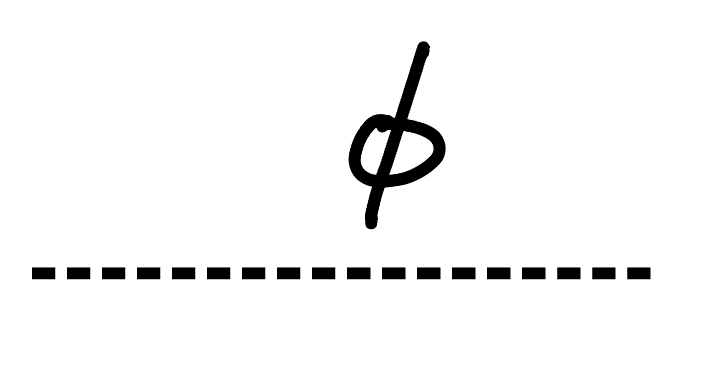
\includegraphics[width=0.2\linewidth]{KG_prop.jpeg} & $\frac{i}{p^2 - m^2 + i \epsilon}$ \\
    \hline
    Propagator & 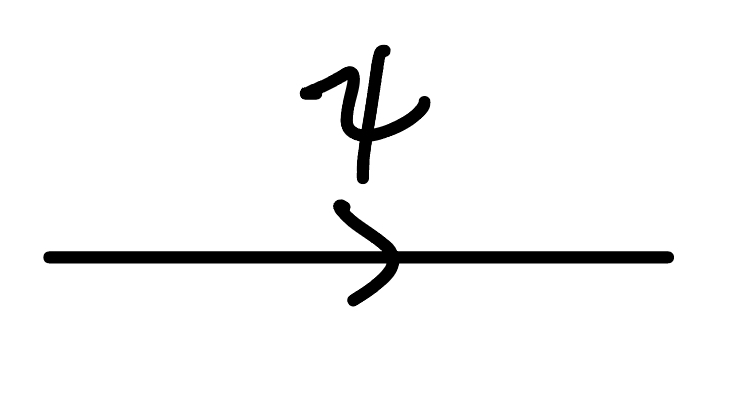
\includegraphics[width=0.2\linewidth]{D_prop.jpeg} & $\frac{i( \slashed{p} + M )}{p^2 - M^2 + i \epsilon}$ \\
    \hline
    Vertex & 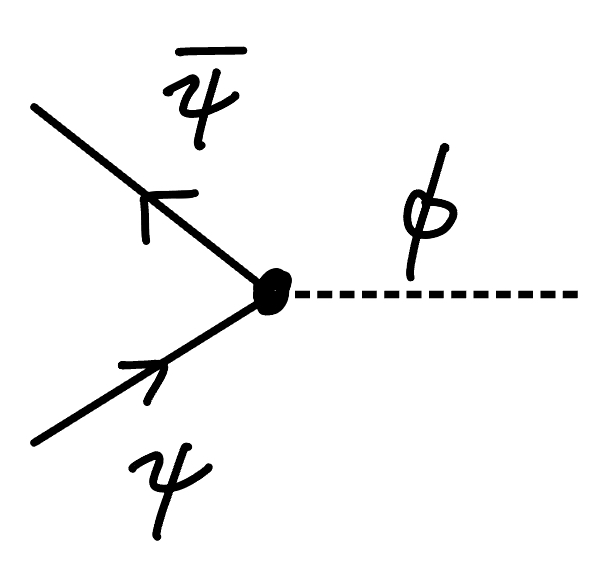
\includegraphics[width=0.2\linewidth]{Y_int1.jpeg} & $- i g$ \\
    \hline
    Vertex & 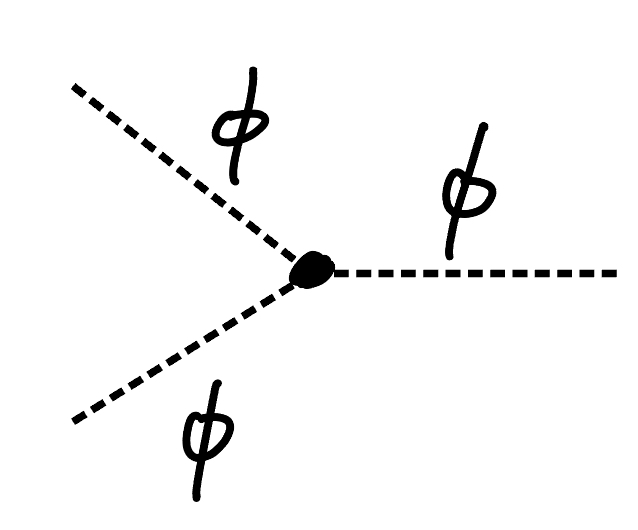
\includegraphics[width=0.2\linewidth]{Y_int2.jpeg} & $- i \lambda_1$ \\
    \hline
    Vertex & 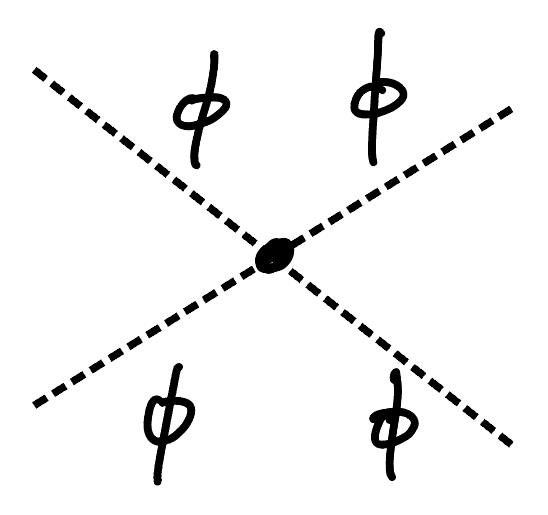
\includegraphics[width=0.2\linewidth]{Y_int3.jpeg} & $- i \lambda_2$
\end{tabular}
\end{table}


}
    
\end{document}
